
%%%%%%%%%%%%%%%%%%%%%%%%%%%%%%%%%%%%%%%%%%%%%%%%%%%
%% Capítulo 1: El Concepto de Fractal
%%%%%%%%%%%%%%%%%%%%%%%%%%%%%%%%%%%%%%%%%%%%%%%%%%%


Las primeras preguntas que se pueden plantear son ¿qué es un fractal? ¿Qué tienen de especial estas figuras? ¿Qué las diferencia de un objeto no fractal? ¿Por qué es necesaria una geometría fractal? Trataremos de responder a cada una de estas preguntas a lo largo de este capítulo, comenzando por la primera de ellas. En realidad, hay distintas definiciones de \textit{fractal}, pero todas utilizan dos conceptos como base: la \textbf{autosimilaridad} y la \textbf{dimensión}. La primera de ellas es más cercana para nosotros de lo que en un principio podemos pensar, fijémonos en los ejemplos de la imagen \ref{fig:objetos}. 

\begin{figure}[h]
\begin{tabular}{cc}
  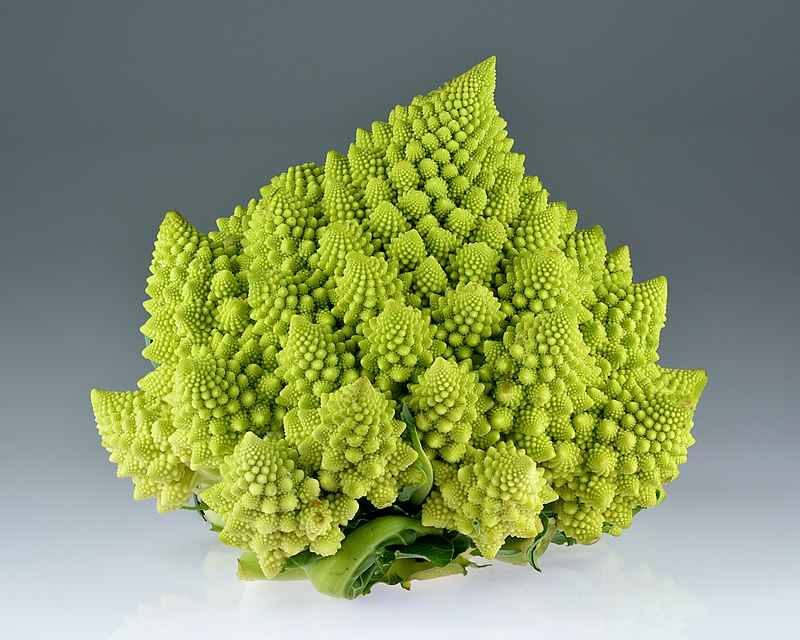
\includegraphics[scale=0.24]{./img/romanescu.jpg} &   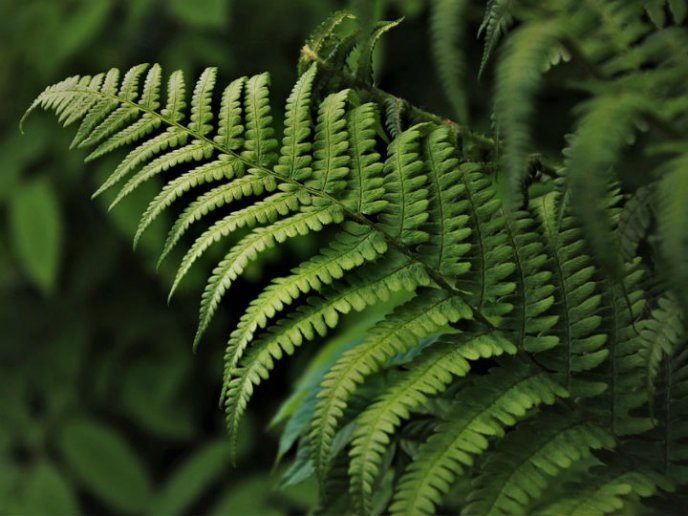
\includegraphics[scale=0.28]{./img/helecho.jpg} \\
(a) Romanescu & (b) Hoja de un helecho \\[6pt]
\end{tabular}
\caption{Objetos cotidianos con estructura fractal}
\label{fig:objetos}
\end{figure}

Observemos que el romanescu, que es un tipo de coliflor, pareciera que está formado de pequeños trozos que recuerdan el objeto original, mientras que estos pequeños trozos a su vez también están formados de pequeños trozos que recuerdan al original, y así sucesivamente. Por su parte, la hoja de un helecho también pareciera estar formada por muchas hojas más pequeñas similares a la original, y estas pequeñas hojas a su vez también están formadas por otras hojas aún más pequeñas.

Esta idea de objetos prácticamente iguales al original salvo cambios de escala es la subyacente al concepto de autosimilaridad.

\begin{definicion}[Autosimilaridad] Una figura o subconjunto $A$ de $\R^n$ es \textbf{autosimilar} si está compuesto por copias de sí mismo reducidas mediante un factor de escala. Es decir,
$$
A = \bigcup_{i=1}^n h_i(A),
$$
donde cada $h_i, i=1,\dots,n$ es una homotecia de razón menor que 1. 
\end{definicion}

En futuras ocasiones se utilizarán indistintamente los términos de <<reducción por un factor de escala>> e <<imagen vía una homotecia>>, queriendo en ambos casos referirnos a este concepto.

Para afianzar y formalizar conceptos y con el objetivo de introducir un concepto de dimensión, estudiaremos algunos ejemplos clásicos de objetos fractales.

\section{Ejemplos clásicos}
\label{section:ejemplos}

\subsection{El conjunto de Cantor}
\label{subsection:Cantor}

Creado por el célebre matemático \textit{George Cantor}, este fractal se construye a partir de un segmento de línea recta aplicando el siguiente proceso iterativo:

\begin{enumerate}
\item Partimos del segmento de recta compuesto por el intervalo cerrado $[0,1]$, aunque realmente es indiferente qué intervalo se escoja, pues el resultado final será el mismo salvo homotecia. Dividimos dicho segmento en tres segmentos iguales y extraemos el intervalo central, manteniendo los extremos. Es decir, extraemos el intervalo abierto $\left(\frac 1 3, \frac 2 3\right)$ y mantenemos el segmento $\left[0,\frac 1 3\right]$ y el $\left[\frac 2 3, 1\right]$.. Nótese que obtenemos $2=2^1$ segmentos, cada uno a escala $\frac 1 3=\left(\frac 1 3\right)^1$ del original.

\item Aplicamos el mismo proceso a los segmentos $\left[0,\frac 1 3\right]$ y $\left[\frac 2 3, 1\right]$. Esto es, se dividen ambos en tres partes iguales y se extrae el intervalo abierto central de cada uno de ellos, manteniendo los extremos. En este caso obtendríamos $4=2^2$ segmentos iguales, cada uno de ellos a escala $\frac 1 3$ de los dos obtenidos en el primer paso y a escala $\frac 1 9=\left(\frac 1 3\right)^2$ del original.

\item Repetimos este proceso de manera indefinida, de manera que en el $n$-ésimo paso se obtendrían $2^n$ segmentos de recta a escala $\left(\frac 1 3\right)^n$. Denotemos como $C_n$ al conjunto unión de los $2^n$ segmentos de recta que se generan en el paso $n$ del proceso.
\end{enumerate} 

Los puntos del intervalo inicial $[0,1]$ que restan tras las infinitas iteraciones son los que conforman el \textit{conjunto de Cantor}, que denotamos con $\mathbf{C}$, de forma que $\mathbf{C}=\bigcap_{n\in\N}C_n$.

\begin{figure} [h]
\centering
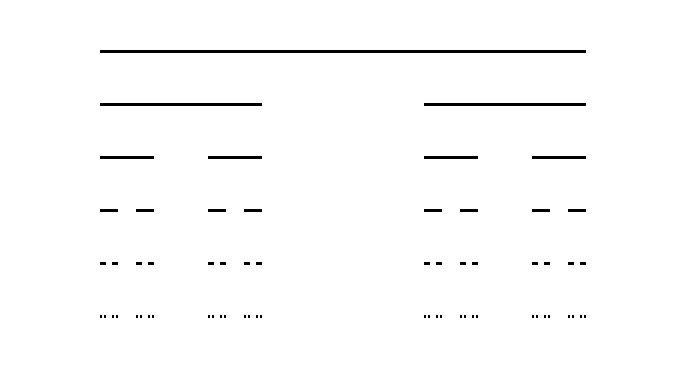
\includegraphics[scale = 0.4]{img/cantor.png}
\caption{Iteraciones del proceso de generación del conjunto de Cantor}
 \label{fig:Cantor}
\end{figure}

El conjunto de Cantor es además un conjunto compacto, pues cada $C_n$ es una unión finita de intervalos cerrados y acotados, y por tanto compactos. Sabiendo que la intersección numerable de conjuntos compactos es compacta, tenemos pues que $\mathbf{C}$ es un conjunto compacto.

\subsection{La curva de Koch}
\label{subsection:curva-Koch}

Esta figura, creada por el sueco \textit{N. F. Helge von Koch} sigue un proceso de construcción iterativo al igual que el conjunto de Cantor, pero en lugar de eliminar segmentos, se añaden de la siguiente manera (ver imagen \ref{fig:curva-Koch})

\begin{enumerate}
\item Partiendo de un segmento de recta de longitud $1$ (al igual que en el conjunto de Cantor, la longitud del segmento inicial es irrelevante, pues la figura final es la misma salvo homotecia), se divide en tres partes iguales de longitud $\frac 1 3$ y la parte central se sustituye por un triángulo equilátero al que se le elimina la base. Esto da lugar a $4=4^1$ segmentos de recta de longitud $\frac 1 3=\left(\frac 1 3\right)^1$.

\item Repetimos este proceso en cada uno de los segmentos de recta obtenidos, colocando el triángulo siempre por encima de la recta, obteniendo así $16=4^2$ segmentos de recta de longitud $\frac 1 9=\left(\frac 1 3\right)^2$.

\item Aplicamos este proceso indefinidamente, obteniendo en el paso $n$-ésimo $4^n$ segmentos de longitud $\left(\frac 1 3\right)^n$. 
\end{enumerate}

El resultado final del proceso es lo que llamamos la \textit{curva de Koch}, que denotamos como \textbf{K}.

\begin{figure} [h]
\centering
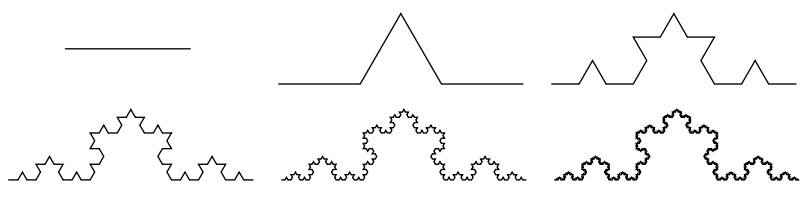
\includegraphics[scale = 0.6]{img/curva-Koch.png}
\caption{Iteraciones del proceso de generación de la curva de Koch}
 \label{fig:curva-Koch}
\end{figure}

\subsection{El copo de nieve de Koch}
\label{subsection:copo-Koch}

A partir de la curva de Koch podemos generar un objeto matemático muy particular: el copo de nieve de Koch. Para crearlo, basta aplicar el proceso iterativo descrito para generar la curva de Koch a cada uno de los segmentos que componen un triángulo equilátero, de forma que los triángulos que se generan apunten hacia el exterior.


\begin{figure} [h]
\centering
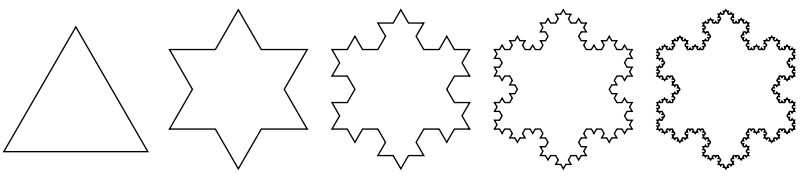
\includegraphics[scale = 0.6]{img/copo-Koch.png}
\caption{Generación del copo de nieve de Koch}
\label{fig:copo-Koch}
\end{figure}

Esta curva posee la particularidad de tener longitud infinita y a su vez encerrar un área finita. Realmente el copo de Koch no es exactamente un fractal, pues no es totalmente autosimilar, aunque se compone de tres partes idénticas las cuales sí son autosimilares, como podemos ver en la imagen \ref{fig:copo-Koch-colores}.

\begin{figure} [h]
\centering
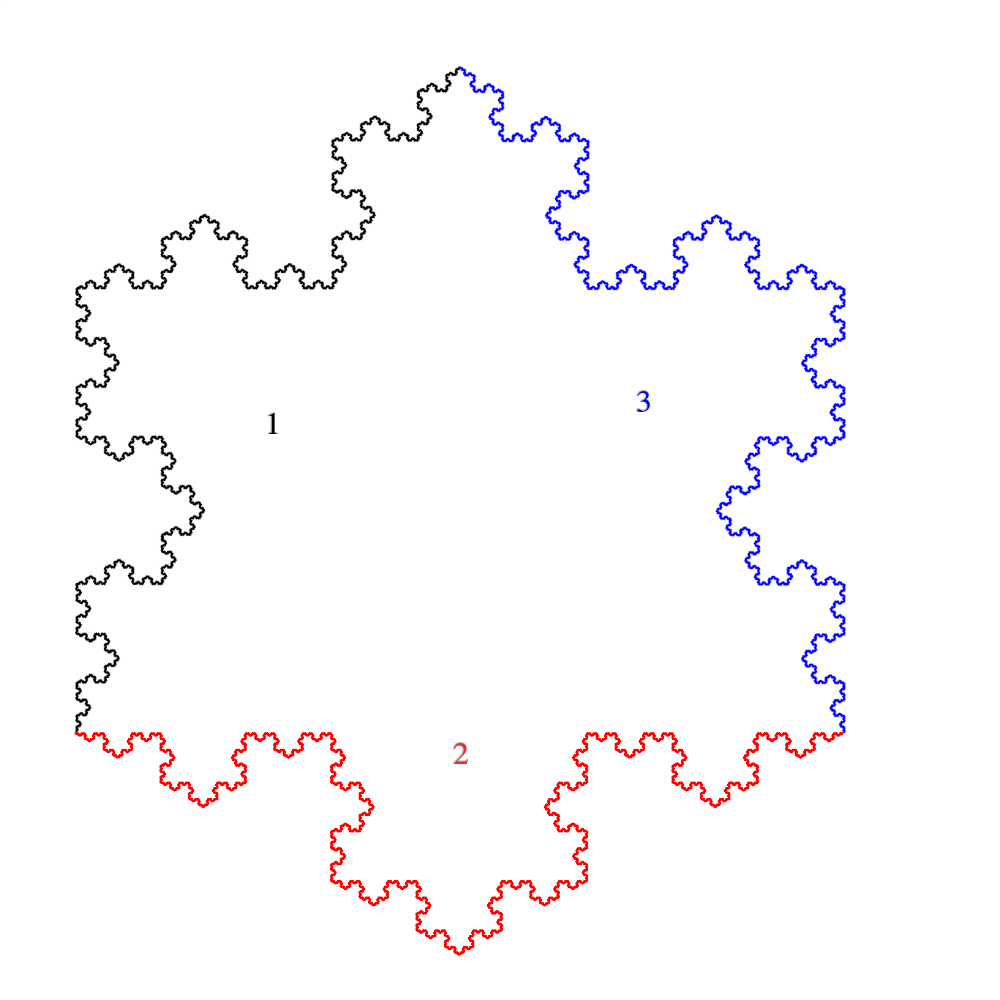
\includegraphics[scale = 0.2]{img/copo-Koch-colores.png}
\caption{Curvas de Koch que componen el copo de Koch}
\label{fig:copo-Koch-colores}
\end{figure}

\subsection{El triángulo de Sierpinski}
\label{subsection:triangulo-Sierpinski} 

Esta figura, original del polaco \textit{Waclaw Sierpinski}, es creada de una manera que evoca al conjunto de Cantor, pero en dos dimensiones. Veamos detalladamente el proceso (ver imagen \ref{fig:triangulo-Sierpinski}):

\begin{enumerate}
\item Se parte de un triángulo equilátero de lado 1 (de nuevo la longitud inicial es irrelevante). Uniendo los puntos medios de cada lado obtenemos una partición del triángulo inicial en 4 triángulos equiláteros, del cual extraemos el interior del triángulo central. Tenemos por tanto $3=3^1$ triángulos a escala $\frac 1 2 = \left(\frac 1 2\right)^1$ del original.

\item En cada uno de estos tres triángulos equiláteros se repite la operación anterior, obteniendo por tanto $9=3^2$ triángulos, cada uno a escala $\frac 1 4 = \left(\frac 1 2\right)^2$ del original.

\item Repetimos este proceso indefinidamente, de forma que en el paso $n$-ésimo se tienen $3^n$ triángulos, cada uno de ellos a escala $\left(\frac 1 2\right)^n$ del original.
\end{enumerate}

La figura a la que converge este proceso infinito se conoce como triángulo \textbf{S} de Sierpinski.

\begin{figure} [h]
\centering
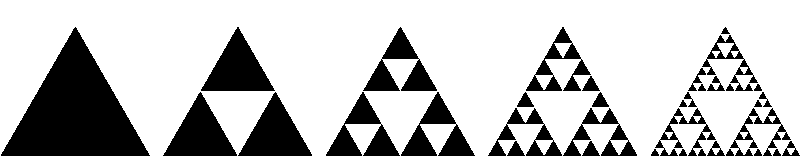
\includegraphics[scale = 0.6]{img/Sierpinski-triangle.png}
\caption{Generación del triángulo de Sierpinski}
 \label{fig:triangulo-Sierpinski}
\end{figure}

Si llamamos $A$ al área del triángulo inicial, sabemos que en la primera iteración eliminamos un área de $\frac 1 4 A$, en el segundo eliminamos $3 \left(\frac 1 4\right)^2 A$ y en el $n$-ésimo $3^{n-1}\left(\frac 1 4\right)^n A$, de forma que si sumamos todo el área que eliminamos en cada paso obtenemos:
$$
A \sum_{n=1}^\infty 3^{n-1}\left(\frac 1 4\right)^n  = \frac A 4  \sum_{n=0}^\infty 3^n\left(\frac 1 4\right)^n =  \frac A 4  \sum_{n=0}^\infty \left(\frac 3 4\right)^n = \frac{A}{4} \left(\frac{1}{1-\frac{3}{4}}\right) = A,
$$
donde hemos usado que la suma de una serie geométrica de razón $|q|<1$ es $\sum_{n=0}^\infty q^n = \frac{1}{1-q}$.

Es decir, el área eliminada es igual al área total y aún así tenemos puntos (por ejemplo los vértices de los triángulos que se van generando). Es decir, los puntos que forman \textbf{S} no están agrupados formando un área.

\subsection{La alfombra de Sierpinski y la esponja de Menger}
\label{subsection:alfombra-esponja}

El propio Sierpinski se dio cuenta que con el mismo patrón utilizado para generar \textbf{S} se pueden generar otras formas. Por ejemplo, pensemos que en lugar de partir de un triángulo equilátero partimos de un cuadrado, lo subdividimos en 9 cuadrados de lado $\frac 1 3$ y extraemos el cuadrado central. Repitiendo este proceso indefinidamente con cada uno de los cuadrados que se generan finalmente se obtiene la llamada alfombra de Sierpinski (ver imagen \ref{fig:alfombra-Sierpinski}).

\begin{figure} [h]
\centering
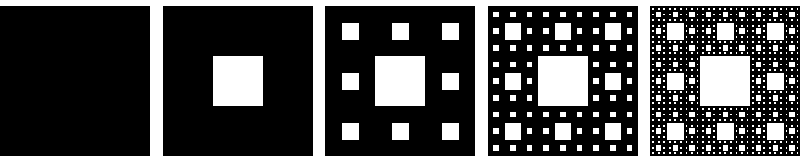
\includegraphics[scale = 0.6]{img/Sierpinski-carpet.png}
\caption{Generación de la alfombra de Sierpinski}
 \label{fig:alfombra-Sierpinski}
\end{figure}

Este proceso también se puede modelar en 3D, obteniendo así la conocida como esponja de Menger o cubo de Magritte, que es una generalización en tres dimensiones de la alfombra de Sierpinski, la cual podemos ver en la imagen \ref{fig:esponja-menger}.

\begin{figure} [h]
\centering
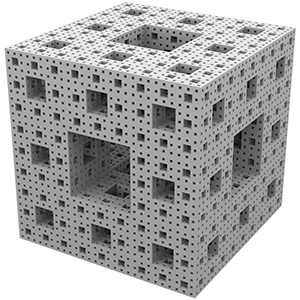
\includegraphics[scale = 0.6]{img/esponja_menger.png}
\caption{Esponja de Menger}
 \label{fig:esponja-menger}
\end{figure}

\section{Conceptos de dimensión fractal}
\label{section:dimension}

Al iniciar este capítulo mencionamos que las distintas definiciones de fractal utilizaban los conceptos de autosimilaridad y dimensión. Con los distintos ejemplos hemos entendido el primero de ellos, por lo que es momento de abordar el concepto de dimensión. 

Intuitivamente, sabemos que una recta o un segmento de recta es de dimensión 1, pues sólo nos podemos mover en una dirección: de derecha a izquierda (el movimiento se describe con un único parámetro). Según este razonamiento y de acuerdo con la intuición un conjunto de puntos aislados es un conjunto de dimensión 0, pues no existe movilidad. Un cuadrado es de dimensión 2, ya que nos podemos mover de izquierda a derecha o de arriba a abajo (el movimiento se describe con dos parámetros: largo y ancho). Un cubo es de dimensión 3 porque en él nos podemos mover de derecha a izquierda, de arriba a abajo o de más a menos profundidad (el movimiento se describe con tres parámetros: altura, anchura y profundidad). 

Pensemos ahora en el triángulo de Sierpinski y en su dimensión. Comprobamos en la sección \ref{subsection:triangulo-Sierpinski} que su área 2-dimensional es nula, pero en el objeto final pareciera que un punto se pudiera mover en varias direcciones. No se puede afirmar que \textbf{S} tenga dimensión 1 por la movilidad, pero tampoco dimensión 2 porque tiene área 0, pero sería un valor situado entre estos dos enteros.

\subsection{Dimension fractal autosimilar}
\label{subsection:dim-frac-autosimilar}

Volvamos a pensar en un segmento de recta, un cuadrado y un cubo, objetos de 1, 2 y 3 dimensiones respectivamente. Supongamos ahora que cada lado de cada objeto se divide en 4 como indica la imagen \ref{fig:divisiones}. Entonces en el segmentro aparecen $N(4):=4=4^1$ segmentos a razón $r=\frac 1 4$ del original, en el cuadrado se obtienen $N(4):=16=4^2$ cuadrados, cada uno a razón $\frac 1 4$ del original y en el cubo $N(4):=64=4^3$ cubos, de nuevo cada uno de ellos a razón $\frac 1 4$ del cubo original.

\begin{figure}[h]
\begin{tabular}{ccc}
  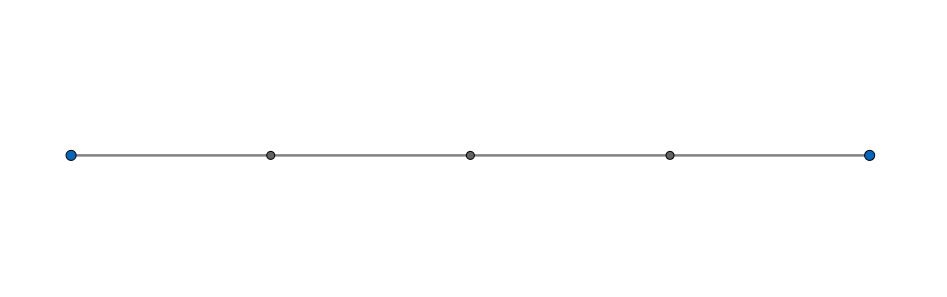
\includegraphics[scale=0.15]{./img/linea-dividida.png} &   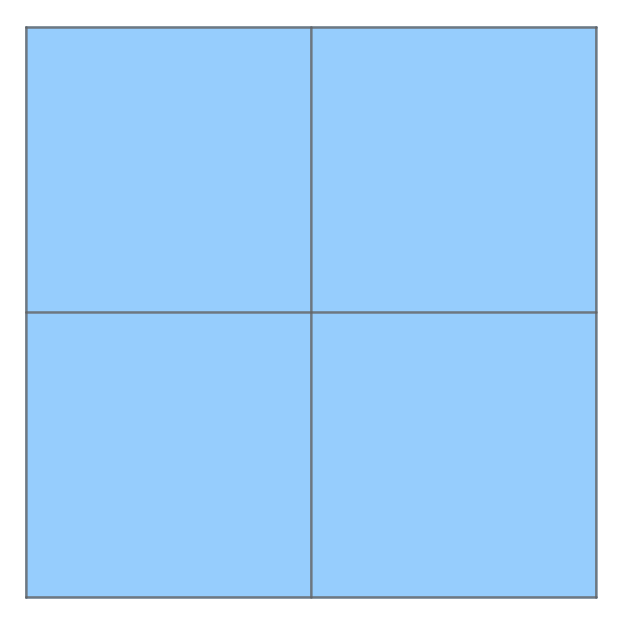
\includegraphics[scale=0.15]{./img/cuadrado-dividido.png} & 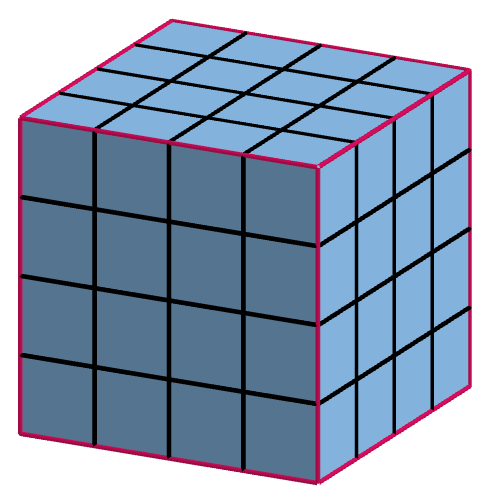
\includegraphics[scale=0.2]{./img/cubo-dividido.png}\\
(a) Segmento dividido en 4 & (b) Cuadrado dividido en 16 & (c) Cubo dividido en 64 \\[4pt]
\end{tabular}
\caption{Segmento, cuadrado y cubo divididos en 4}
\label{fig:divisiones}
\end{figure}

Si en lugar de 4 tomamos cualquier número natural $k\geq 1$, la razón sería $r=\frac 1 k$ y en ese caso se obtendrían $N(k)=k^1$ segmentos de recta, $N(k)=k^2$ cuadrados y $N(k)=k^3$ cubos, en todos los casos a escala $r=\frac 1 k$ de los objetos originales. Estas igualdades se pueden reescribir como:

\begin{equation}\label{eq:relaciones-dimension}
\frac{N(k)}{k^1}=1 \hspace{2cm} \frac{N(k)}{k^2}=1 \hspace{2cm} \frac{N(k)}{k^3}=1
\end{equation}

En este sentido, vemos que la dimensión de cada objeto es el \textit{exponente} al que habría que elevar el factor de contracción $k$ para obtener la relación (\ref{eq:relaciones-dimension}). De manera análoga podemos tomar cualquier figura o subconjunto $X\subseteq \R^n$ que pueda ser subdividido en un número finito $N(k)$ de subfiguras o subconjuntos idénticos salvo traslaciones o rotaciones y que sean una copia a escala $r=\frac 1 k$ del objeto original.

\begin{definicion}[Dimensión autosimilar]
Dado un subconjunto $X$ de $\R^n$ que se puede dividir en $N(k)$ subconjuntos congruentes entre sí e idénticos a $X$ por un factor de escala de $r=\frac 1 k$, definimos su \textbf{dimensión autosimilar} como el único valor $d$ que satisface la identidad $\frac{N(k)}{k^d}=1$, es decir: 
$$
d=\frac{\log N(k)}{\log(k)}
$$
\end{definicion}

\begin{wrapfigure}{l}{0cm}
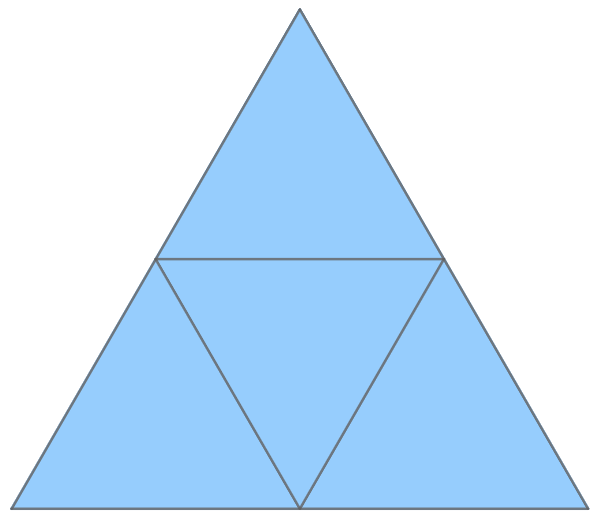
\includegraphics[scale=0.14, trim={0cm 0.35cm 0cm 0.5cm}, clip]{./img/triangulo-dividido.png}
\end{wrapfigure}

Un ejemplo distinto pero clarificador podría ser el de un triángulo equilátero, el cual podemos dividir en 4 copias congruentes entre sí, cada una a escala $r=\frac 1 2$ del triángulo original, de forma que tendríamos $k=2$ y $N(2)=4$. 

Con estos valores, tenemos que $N(k)=4=k^d=2^d$, por lo que necesariamente $d=2$ y por tanto un triángulo equilátero es un objeto 2-dimensional, lo cual tampoco nos sorprende.

\begin{observacion}
La dimensión $d$ ya no tiene por qué ser necesariamente un número entero. A esta posibilidad de tener dimensiones no enteras es a lo que llamamos \textbf{dimensión fractal autosimilar}, y lo denotamos con $D$.
\end{observacion}

Retomando ahora el triángulo de Sierpinski, sabemos que este está compuesto por 3 copias de sí mismo a escala $\frac 1 2$ (véase sección \ref{subsection:triangulo-Sierpinski}), por lo que entonces su dimensión fractal autosimilar es $D=\frac{\log 3}{\log 2} \approx 1.58496$. Efectivamente y tal y como discutimos en el inicio de esta sección, es un valor situado entre 1 y 2.

En cuanto al conjunto de Cantor, este está formado por 2 copias de sí mismo a escala $\frac 1 3$ (sección \ref{subsection:Cantor}), por lo que su dimensión fractal autosimilar sería $D=\frac{\log 2}{\log 3} \approx 0.63093$, que es un valor situado entre 0 y 1.

Por su parte, la curva de Koch se compone de 4 copias de sí misma, cada una a escala $\frac 1 3$ de la curva original (sección \ref{subsection:curva-Koch}). Por tanto, su dimensión fractal autosimilar es $D=\frac{\log 4}{\log 3} \approx 1.26186$.

\subsection{Dimensión por cajas}
\label{subsection:dim-cajas}

El concepto de dimensión fractal autosimilar tiene el defecto de que está limitado únicamente a objetos totalmente autosimilares, pero la mayoría de objetos no cumple esta propiedad. Para solucionar este problema, introduciremos el concepto de dimensión por cajas.

Dada una figura o conjunto $A\subset \R^2$, lo recubrimos con una cuadrícula en la que todos los cuadrados son iguales, de longitud $\delta$. A estos cuadrados los llamamos \textit{cajas}. Contamos los cuadrados necesarios para recubrir la figura, obteniendo el número $N_\delta(A)$, que es dependiente de la longitud de los cuadrados. Si disminuimos el valor $\delta$ obtendríamos un número posiblemente distinto y más óptimo de cuadrados necesarios para recubrir la figura. Notemos que este proceso de hecho se puede generalizar a tres dimensiones si usamos cubos de lado $\delta$ en lugar de cuadrados.

\begin{definicion}[Dimensión por cajas]
Se define la \textbf{dimensión por cajas} de un subconjunto $A\subset \R^2$, denotada por $D(A)$ como:

\begin{equation}\label{eq:dim-cajas}
D(A)=\lim_{\delta\rightarrow\infty}\frac{\log N_\delta(A)}{\log(1/\delta)}
\end{equation}

\end{definicion}

\subsection{Dimensión de Hausdorff}
\label{subsection:dim-Hausdorff}

La dimensión por cajas tiene el inconveniente de que no tenemos garantizada la existencia de límite en la ecuación (\ref{eq:dim-cajas}) o hipotéticos problemas con conjuntos más generales, por ejemplo conjuntos densos. Por ejemplo, $\Q\times\Q\subset\R^2$ es un conjunto denso pero numerable, su dimensión debería ser 0. Para solucionar estos problemas \textit{Felix Hausdorff} publicó en 1918 un artículo que cambiaría la teoría de la medida tal y como la conocíamos. 

Supongamos que queremos medir el área de un conjunto $A\subset\R^2$ complicado, como podría ser el triángulo de Sierpinski. Una manera de hacerlo es recubrir $A$ con una sucesión de discos $D_1,D_2,\dots$. Entonces el área de $A$ está acotada superiormente por la suma de las áreas de todos estos discos:
\begin{equation}\label{eq:cota-A}
\lambda_2(A)\leq \frac \pi 4 \sum_{n\in\N}\diam(D_n)^2
\end{equation}

donde $\lambda_2$ denota la medida 2-dimensional de Lebesgue.

Sin embargo en esta aproximación la cota es demasiado grande, aunque podemos refinarla usando otros discos cada vez más pequeños, siempre que recubran a $A$. De esta forma, el área de $A$ será el valor más pequeño que podamos obtener con cualquier sucesión de discos al sumar sus áreas como en (\ref{eq:cota-A}).
\begin{equation}
\lambda_2(A)=\inf\left\lbrace \frac \pi 4 \sum_{n\in\N}\diam(D_n)^2 \ | \  D_1,D_2,\dots \text{ recubren a A }\right\rbrace
\end{equation}

Si como ejemplo aplicamos esta definición a un segmento de recta, el cual podemos recubrir con $n$ circunferencias de diámetro $\frac 1 n$, tendríamos aplicando (\ref{eq:cota-A}) que el área está acotada por $\frac \pi 4 \cdot n \cdot \left(\frac 1 n\right)^2=\frac c n$, donde $c$ es una constante positiva. Tomando círculos cada vez más pequeños, es decir, tomando límite en $n$, tenemos que $0 \leq \lambda_2(A) \leq \lim_{n\rightarrow\infty}\frac c n = 0$, obteniendo así que el área 2-dimensional de un segmento de recta es 0, tal y como cabía esperar.

Para calcular la medida 1-dimensional (i.e. la longitud) de $A$ aplicamos el mismo proceso pero en lugar de calcular la suma de las áreas podemos calcular la suma de los diámetros de los discos, es decir:

$$
\lambda_1(A)\leq\sum_{n\in\N}\diam(D_n) 
$$
$$
\lambda_1(A)=\inf\left\lbrace \sum_{n\in\N}\diam(D_n) \ | \  D_1,D_2,\dots \text{ recubren a A }\right\rbrace 
$$

Por tanto, la medida $d$-dimensional de $A$ será \footnote{Recordemos que el símbolo $\propto$ denota proporcionalidad.}
\begin{equation}\label{ec:medida-d-dimensional}
\lambda_d(A)\propto \inf\left\lbrace \sum_{n\in\N}\diam(D_n)^d \ | \  D_1,D_2,\dots \text{ recubren a A }\right\rbrace
\end{equation}

Por comodidad y simplicidad, en la práctica se usan círculos de igual radio, digamos $\varepsilon\geq 0$, y se asume que $A$ es un subconjunto cerrado y acotado de $\R^2$. Llamamos $N_\varepsilon(A)$ al número de círculos de radio $\varepsilon$ necesarios para recubrir a $A$, de forma entonces que según (\ref{ec:medida-d-dimensional}) la medida $d$-dimensional de un conjunto $A\subset\R^2$ es proporcional a
\begin{equation}
h^d(A):= \lim_{\varepsilon\rightarrow 0} N_\varepsilon(A)\varepsilon^d
\end{equation}

Sin embargo, para poder calcular estas medidas necesitamos asegurarnos la existencia de este límite para algún valor de $d$.

\begin{teorema}
\label{th:Hausdorff}
Sea $A\subset \R^n$ un conjunto cerrado y acotado. Entonces existe un único valor de $d$ para el cual $h^d(A)$ no es ni $0$ ni $\infty$. Este valor $d=D_H(A)$ satisface que:
\begin{equation}
h^d(A)= \left\{ \begin{array}{lcc}
             \infty &   si  & d < D_H(A) \\
             \\ 0 &  si & d > D_H(A) 
             \end{array}
   \right.
\end{equation}
\end{teorema} 

\begin{definicion}[Dimensión de Hausdorff]
Llamamos \textbf{dimensión de Hausdorff} de un conjunto $A$ al único valor $D_H(A)$ del teorema \ref{th:Hausdorff}.
\end{definicion}

De manera natural, para objetos autosimilares los conceptos de dimensión fractal autosimilar y dimensión de Hausdorff coinciden.


\subsection{Dimensión topológica}

Por último estudiaremos un concepto de dimensión aplicable a espacios topológicos. La \textbf{dimensión topológica} se define inductivamente de la siguiente forma:

\begin{enumerate}
\item La dimensión del conjunto vacío es $\partial(\emptyset):=-1$.
\item Un espacio topológico $X$ tiene dimensión 0 ($\dim(X)=0$) si para cualquier $x\in V$ con $V$ abierto en $X$ existe un abierto $U$ cuya frontera $\partial(U)$ es vacía y se verifica que $x\in U\subseteq V$.

\item Un espacio topológico $X$ tiene dimensión menor o igual que $n$ ($\dim(X)\leq n$) si para cualquier $x\in X$ y cualquier $V$ abierto que contiene a $x$ existe un abierto $U$ tal que $\dim(\partial(U))\leq n-1$ y se verifica que $x\in U\subseteq V$. 

\item $X$ tiene dimensión $n$ ($\dim(X)=n$) si se verifica que $\dim(X)\leq n$ pero es falso que $\dim(X)\leq n-1$
\end{enumerate}

\begin{figure}[h]
\begin{tabular}{cc}
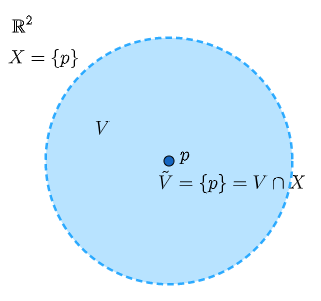
\includegraphics[scale=0.5]{./img/ejemplo-dimension-1.png} &   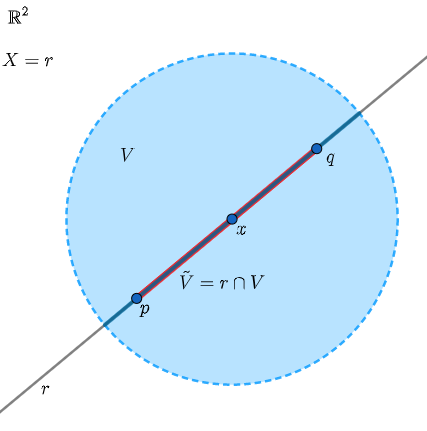
\includegraphics[scale=0.45]{./img/ejemplo-dimension-2.png} \\
(a) Ejemplo con $X=\{p\}$ & (b) Ejemplo con $X=r$ \\[6pt]
\end{tabular}
\caption{Figuras representativas de los ejemplos}
\label{fig:ejemplos}
\end{figure}


\begin{ejemplo}
\label{ej:dimension-1}
(Véase imagen \ref{fig:ejemplos} (a))
En $\R^2$ dotado de la topología usual consideramos un punto $p$ cualquiera y el espacio topológico $X=\{p\}$. Por tanto la topología inducida por la topología usual $\tau$ en $X$ es $\tau_X=\{X,\emptyset\}$. Sea $V$ un abierto de $\R^2$ que contenga a $p$, por tanto $\tilde{V} = V \cap X = \{p\}$ es un abierto en $X$ que contiene a $p$. Podemos encontrar entonces un abierto $U=\{p\}$ de $X$ tal que su frontera $\partial(U)=\emptyset$ y además $p\in U \subseteq V$. Por tanto concluimos que $X$ tiene dimensión 0.
\end{ejemplo}

\begin{ejemplo}
(Véase imagen \ref{fig:ejemplos} (b))
En $\R^2$ dotado de la topología usual, consideramos una recta cualquiera, llamémosla $r$, y el espacio topológico $X=\{r\}$. Sea $x\in X$ y $V$ un abierto de $\R^2$ que contenga a $x$, de forma que $\tilde{V} = r\cap V$ es un abierto de $X$. Podemos entonces tomar un abierto $U$ dentro de $\tilde{V}$ (un segmento abierto de recta), de forma que $x\in U\subseteq \tilde{V}$. Por otro lado, $\partial(U)=\{p,q\}$, y podemos comprobar fácilmente (con ayuda del ejemplo \ref{ej:dimension-1}) que $\dim(\partial(U))=0$. Por todo esto podemos concluir que $X=r$ es un espacio topológico de dimensión 1. 
\end{ejemplo}

A partir de esta definición, la cual notamos que solo puede tomar valores enteros, podemos enunciar nuestra primera definición de fractal, que fue formulada por \textit{Benoit Mandelbrot}.

\begin{definicion}[Fractal]
\label{def:fractal}
Un \textbf{fractal} es un subconjunto del plano que es autosimilar y cuya dimensión fractal excede a su dimensión topológica.
\end{definicion}
